%\chapter[The ILC]{The future of high-energy physics: the International Linear Collider}
\chapter{Towards a linear future: the International Linear Collider}
\label{chap:ILC}

  Since 2008, the \gls{LHC} is the most powerful tool in high-energy physics.
  It will provide a better understanding of the universe, particularly with the discovery in 2012 of a new particle compatible with the Higgs boson responsible for the spontaneous symmetry breaking of the \acrfull{SM} \cite{Aad2012, Chatrchyan2012}.
  Although the \gls{LHC} is an impressive machine able to collide protons at a centre-of-mass energy of $13~\rm{TeV}$, the complex environment of the events makes more difficult to access some fundamental parameters. 
  To test the validity of the \gls{SM} and other physics theories introduced in chapter~\ref{chap:SM}, the high-energy physics community has converged on the necessity to build a linear electron-positron collider.
  
  This chapter will explain the motivations to invest into a new global project. 
  It will present the complementary nature of the lepton and hadron colliders and the main advantages of lepton collisions will be discussed.
  After giving an overview of the \gls{ILC} with its basic design and the detector models, we will focus on the design of one of the detectors: the \gls{ILD}.

 \minitoc
  
  \section{Towards a linear electron collider}
 
  The most impressive accelerator ever built is located at \gls{CERN} in Geneva, Switzerland. 
  It is the world's largest particle accelerator, with a circumference of nearly 27 kilometers, straddling the Swiss and French border.
  It is designed to collide two beams of protons or heavy ions, with the possibility to reach centre-of-mass energies of $13~\rm{TeV}$ with a peak luminosity of $10^{34}~\rm{cm}^2\rm{.s}^{-1}$.
  The goals of the \gls{LHC} are to perform tests of the \gls{SM} and to search for new forces and/or particles. 
  The collider covers a wide energy range at the constituent level while running at a fixed beam energy.
  Nevertheless, the particles used for the collision are not elementary ones, thus, the measurements are impacted by the hadronic background produced.
  
  A machine dedicated to precision measurements, complementary to the \gls{LHC}, would bring very valuable to the physics community.
  The advantages of linear electron collider will be presented in the following.

    \subsection{Advantages of a linear lepton collider}
    \label{subsec:advLLC}
    
    First of all, in a hadron collider because of the compositeness of the particles used, only a part of the total centre-of-mass energy is used during each collision.
    The four-vector momentum  of the interacting particles is not known because of the unknown number of partons part of the interaction.
    By colliding leptons, which are structureless objects, the full centre-of-mass energy is available for the elementary process. 
    The initial four-vector momentum of an interaction is exactly known, hence the event is fully reconstructed.

    Secondly, with a lepton collider, the beam energy is tunable and both electron and positron beams can be polarised. 
    The spin of the initial state is known.
    The selection of an appropriate polarisation can enhance the signal and suppress the background. 

    Thirdly, the proton-proton interaction cross section is dominated by inelastic background QCD processes.
    The signal event is then accompanied by large backgrounds produced by the bunches interaction.
    This background masks the elementary process of interests, such that it has an impact on the detector design, that should have a high radiation tolerance and implement a selective trigger to reduce the data rate.
    The lepton colliders do not suffer from this kind of background and at similar energies, the event rate is lower than those at hadron colliders.
    Moreover, the interaction of electrons and positrons is purely electroweak.
    In consequence, the detector does not have to handle extreme data rates and can be used without any trigger.
    Hence, the sensitivity to any possible signature of new physics is improved.\todo{REPHRASE EVERYTHING}

    Although the electron and positron, have clear advantages over hadrons to perform precise measurements, the choice of a linear collider over a circular one comes from the physics of accelerating charged particles.
    When charged particles move in a circular accelerator, they lose some energy by emitting photons via synchrotron radiation.
    Equation~\ref{eq:Esynchrotron} describes this energy loss:
    
    \begin{equation}
     \Delta E_{\rm{sync}} \sim \frac{E^4}{m^4r}.
       \label{eq:Esynchrotron}
    \end{equation} 

    The radiative energy loss $\Delta E_{\rm{sync}}$ is inversely proportional to the radius $r$ of accelerator, the energy of the particle $E$ to the power of the fourth and its mass $m$ to the power of the fourth.
    As the electron mass is $\sim 1.8 \times 10^3$ smaller than the proton mass, the energy loss radiated by the electron is much higher than the energy loss radiated by proton at the same centre-of-mass energy.
    To compensate the energy loss, a circular electron-positron accelerator should have an extremely large radius (larger than the actual \gls{LHC}), increasing the cost to build the experiment.
    Another solution to overcome the synchrotron radiation is to accelerate the particles in a linear collider.
    The centre-of-mass energy has to be reached only passing once through the accelerator, whereas a bunch of particles in a circular collider is accelerated many times until the desired energy of collision is reached.
    The choice of a linear collider over a circular one comes also from the cost, which has a quadratic energy dependence for a circular one, whereas it follows a first power energy for a linear one \cite{Richter:1976ug}. 
    %To still get an "affordable" experiment, the centre-of-mass energy obtained at a linear collider is below to the one from a circular collider.\todo{WRONG: read B.Richter paper on SLAC} 
    To work at the same energy scale, a linear collider would require a bigger number of accelerating cavities and would make a much bigger and more expensive collider than a circular one.

    \subsection{Future linear lepton collider}
    
    Since the 1980's, several linear collider technologies have been developed, leading in the 1990's to five major accelerator technologies: \gls{SRF}, the \gls{CLIC} technology and three different normal conducting technologies (S-band, C-band, and X-band) \cite{Desy1988}.
    Different projects are under studied for the next high-energy physics experiment. 
    All the projects aim to perform precise measurements.
    CERN is preparing a electron/positron linear collider, called \gls{CLIC}.
    It has a challenging technology to aim a nominal energy of $3~\rm{TeV}$.
    The accelerator will use radio-frequency structures and a two beam concept \cite{CLIC}.
    Another idea would be to develop a muon collider instead of electron-positron collider \cite{Lipton2012}.
    As the electron, the muon is a pointlike particle, therefore the centre-of-mass energy can be easily adjusted to perform a precise study.
    The muon mass is 207 times larger than the electron mass, which means that a muon beam would suffer less energy loss by synchrotron radiation.
    Hence, a muon circular collider could be feasible.
    However, the muon has a lifetime of only $2.2~\rm{\mu s}$ making up a more challenging acceleration design.
 
    At the beginning of the 2000's, the \gls{ICFA} was formed and has chosen in 2004 the \gls{SRF} technology \cite{ICFA2004} to build the \gls{ILC} \cite{ILC}.
    The technology developed for this future experiment is also used for the XFEL at \gls{DESY} in Hamburg and at KEK in Japan.
        
    The \gls{CLIC} and muon colliders will not be described further in this thesis.
     
  \section{The ILC machine}
  
    The \gls{ILC} should be the next lepton collider experiment and will be situated in Japan.
    In 2016, the physics community was waiting for an official decision of the Japan government concerning the final experimental site. \todo{Reference to the decision but which one?}
    At the time when this thesis was written, the scientific community has chosen a site candidate in the north of Japan, in the region of Kitakami. 
    
    \subsection{Baseline design}

   \begin{figure}[!h]
      \centering
      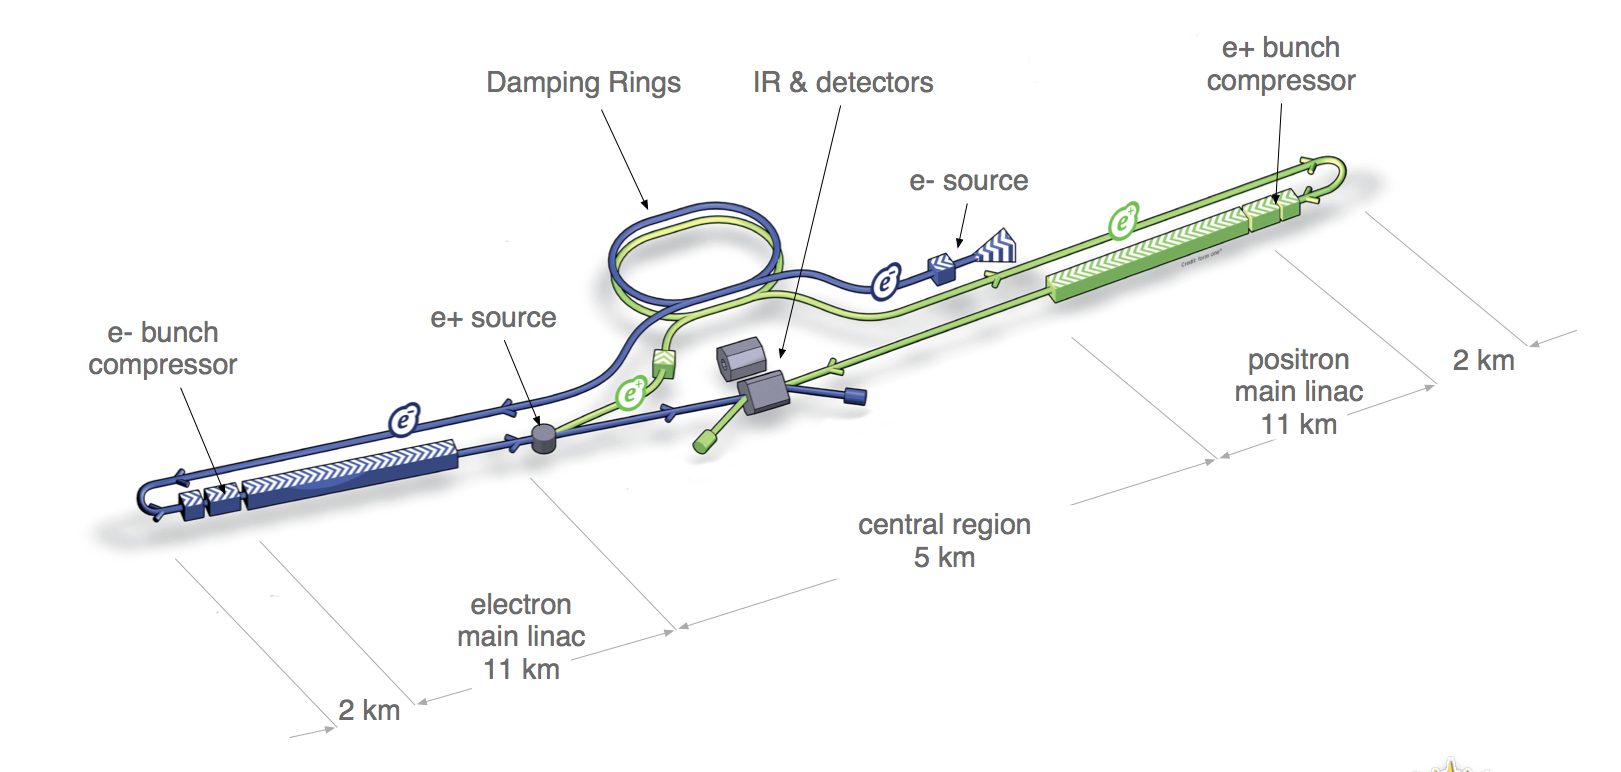
\includegraphics[width = 16 cm]{Pictures/ILC/ILC_new.png}
      \caption{Schematic layout of the International Linear Collider (ILC) \cite{Behnke2013}.}
      \label{fig:ILC}
    \end{figure}


    The \gls{ILC} is planned to collide electrons and positrons at the center-of-mass energies varying between $250~\rm{GeV}$ and $500~\rm{GeV}$ for 31 kilometers long accelerator. 
    An upgrade to reach the centre-of-mass energy of $1~\rm{TeV}$ is possible, but the accelerator will have to be extended to achieve a total length of 50 kilometers.
    It is designed to generate a total of $500~\rm{fb}^{-1}$ of data during the first four years of operation. 
    The luminosity will reach a peak of $2 \times 10^{34}~\rm{cm}^{-2}\rm{.s}^{-1}$ at $\sqrt s = 500~\rm{GeV}$.

    The main components of the \gls{ILC} are presented in the following order.
    An overview of the electron source and their acceleration via the conducting and superconducting structures is presented, then the role of the damping rings, the injection into the main linacs, followed by the positron source and the \gls{BDS} are described.
    Finally, the \gls{IR} is presented.
    A detailed description of the \gls{ILC} can be found in the Technical Design Report \cite{Appleby2006}.

    \subsection{Machine design and beam parameters}
    \label{subsec:design}

    Polarised electrons are produced by a laser firing into strained GaAs photocathode in a \gls{DC} gun.
    To implement a redundancy, the electron generation system is made of two lasers and \gls{DC} guns, providing bunches with a polarisation of $90~\%$.
    The electrons are then pre-accelerated to $76~\rm{MeV}$ using non-superconducting accelerating structures.
    They are then injected into a $250~\rm{m}$ long superconducting linac to reach the energy of $5~\rm{GeV}$.
    The dimension and density of the bunches are quite extended, thus their emittance is too wide.
    Before injecting the bunches into a damping ring, which is used to decrease the emittance and reach the desired luminosity, superconducting solenoids rotate the spin vector into the vertical direction, while \gls{SRF} cryomodules are used for an energy compression.
 
    The damping ring has a $6.7~\rm{km}$ circumference and is made of magnets and wrigglers that are going to force the particles to get a bent track.
    This system is used to dump the electrons with large transverse and longitudinal emittance to the low emittance required for the luminosity production.
    The reduction of the emittance should be achieved within $200~\rm{ms}$ between the machine pulses.
    Although the positron source was not yet introduced, their bunches suffer from the same problems as the electron ones. 
    A second damping ring, placed in the same cavern as the electron one, is also in charge to get the desired emittance.

    The bunches are then extracted from the damping rings and transferred via the \gls{RTML} structure, the longest continuous beam line at the \gls{ILC}.
    It is divided into five subsystems to transport the bunches from the damping rings to the \gls{BDS}.
    It is orienting the beam into the desired polarisation by rotating the spin of the particle.
    The beam bunch length is compressed  from several millimeters to a few hundred by using a two-stage bunch compressor.
     %in order to orient the beam in the desired polarisation by rotating the spin of the particle, but also to compress the beam bunch length from several millimeters to a few hundred microns thanks to a two-stage bunch compressor.
    While the bunches are compressed, sections of \gls{SRF} technology accelerate the bunches from $5~\rm{GeV}$ up to $15~\rm{GeV}$.
    One of the challenges of the \gls{RTML} is to preserve the emittance obtained after the damping rings, while the length and the energy of the bunches are tuned.
    Then, the particles are delivered to the main linac, an 11 km long accelerator using $1.3~\rm{GHz}$ \gls{SRF} cavities, made of niobium.\todo{What are the others made of?}

    Before reaching the interaction region, the primary electron beam is transported through a 147 m superconducting helical undulator to produce photons from $\sim 10$ up to $\sim 30~\rm{MeV}$, depending on the energy of the primary beam.
    This primary beam is separated from the photons and sent back to the \gls{BDS} with an energy loss of $\sim 3~\rm{GeV}$.
    The photons are directed onto a rotating Ti-alloy target to create $e^+e^-$ pairs that are separated.
    The positrons collected are accelerated to $125~\rm{MeV}$ using a normal conducting linac and then accelerated to $5~\rm{GeV}$ with a superconducting boost linac.
    Finally, they are injected into the damping ring to reduce their emittance.

    The two beams are transported from the high energy linacs to the \gls{IR} by the \gls{BDS}, in charge to focus the beams to the sizes required to meet the desired luminosity.
    It is divided into five main subsystems. 
    In the direction of the beam, a system is in charge to perform some emittance measurement and matching, to give a trajectory feedback, and provide a polarimetry and energy diagnostic. 
    Then, the beam is collimated to remove the beam-halo particles that would generate a huge amount of background in the detector.
    Muons generated during the collimation process are deflected by magnetised iron shielding.
    Thereafter, strong compact quadrupoles focus the beam to the sizes required to meet the desired luminosity. 
    Before the collisions, crab cavities rotate the bunches in the horizontal plane for effective collisions and to achieve a 14 mrad total crossing angle.
    After the collisions, an extraction line is dedicated to transport the beams into the main beam dump.

    Although two experiments will run at the \gls{ILC}, there will be only one interaction region due to cost reasons.
    To have two experiments running at the same time, it requires two separate \gls{BDS} of 4 km long each.
    Thanks to a push-pull scheme, the detectors will work alternatively: while one is taking data, the other one is sitting in the garage for maintenance.
    The two detectors will be presented in more details in section~\ref{sec:detectors}.
    
    \begin{figure}[!h]
      \centering
      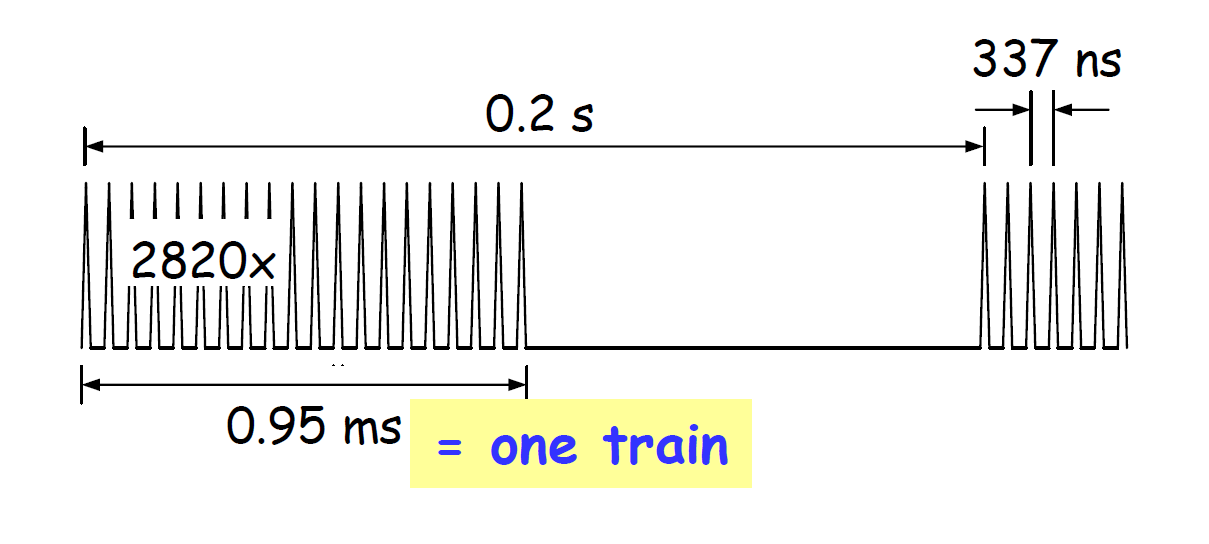
\includegraphics[width = 10cm]{Pictures/ILC/bunch.png}
      \caption{Schematic view of the bunch structure at the ILC. One bunch train is made of 2625 bunches and lasts $0.95~\rm{ms}$. Each bunch crossing is spaced out by $337~\rm{ns}$. Two bunch trains are $0.2~\rm{s}$ apart from each other \cite{Li2010}.}
      \label{fig:bunches}
    \end{figure}

    The accelerator described above will create bunch trains at a repetition rate of $5~\rm{Hz}$. 
    Each train is composed of 2625 bunches that contain $2\times 10^{10}$ particles and lasts $0.95~\rm{ms}$. 
    The interval between two trains is $2~\rm{ms}$ long. 
    This structure is a key feature to develop detectors able to be switched off during the dead time in order to reduce the power consumption.
    \todo{Write TDR values, see Marcel's talk}

    \subsection{Beam backgrounds}

    To design the detectors of the \gls{ILC}, the backgrounds must be understood and taken into account to give optimal performances.
    The event reconstruction becomes more complicated with hits caused by background particles.
    Their are two kinds of background, the one created by the \gls{BDS} and the one related to the interaction point.
    As it was discussed in subsection~\ref{subsec:design}, the collimator placed closed to the \gls{IP} to remove the beam halo, that can produce muons by an electromagnetic shower.
    To sweep them away, iron spoilers are used to create a magnetic field and deflect the muons.
    A side effect is to increase the number of neutrons created in photo-nuclear reactions.
    A concrete wall placed at the entrance of the experimental hall vanishes the neutron background.

    Contrary to the \gls{LHC}, the \gls{ILC} will not suffer from QCD background, as mentioned in section~\ref{subsec:advLLC}.
    Nevertheless, due to the nature of electrons and positrons, the two beams will interact each other before they collide.
    The electromagnetic beam field of each bunch is high and causes the focusing of the opposite bunch.
    It is bending the electron/positron trajectories near the \gls{IP}.
    On the one hand, this effect helps to focus the incoming beams and enhance the luminosity.
    On the other hand, as the charged particles have bending track, they are emitting hard photons via beamstrahlung, creating $e^+e^-$ pairs background.
    The hard photon is strongly focused in the forward region and do not contribute strongly to the background in the detector.
    However, the $e^+e^-$ pairs created contribute to the background directly or through backscattered particles.
    In consequence of the beamstrahlung, the beam particle energy is reduced, hence the collisions occur at different energies from the nominal one and this affects the physics cross-section.
    The beamstrahlung photons can also produce neutrons by hitting components.
    The other source of hard photons is the initial state radiation. 
    With the beamstrahlung, they contribute reducing the luminosity \cite{Markin2014}.
    \todo{Peak luminosity may-be?!}

    Different kinds of soft pairs background can be expected at the \gls{ILC}: the coherent and incoherent pair production.
    The coherent pair production appears when beamstrahlung photons are interacting with the strong electromagnetic field of the beams.
    In the \gls{ILC} environment the coherent pair background are negligible, whereas the incoherent pair production is dominant.
    It corresponds to $e^+e^-$ pairs created by the interaction of only two particles.
    They are to the number of three depending on the nature of the scattered photons creating the $e^+e^-$ pair.
    The Bethe-Heitler process corresponds to the scattering of one real photon while the second one is virtual.
    It contributes to approximately two of the third pair production.
    The second process is the Landau-Lifshitz, where the two scattered photons are virtuals and contribute to approximately to a third of the pair creation.\todo{Sentence not clear}
    The last production occurred via two real photons (Breit-Wheeler process) and contribute only to a percent level.
    The incoherent $e^+e^-$ pairs are produced at a relatively low transverse momentum and are emitted in the forward direction.
    
    %This interaction is called the beamstrahlung and is due to the electromagnetic force which bends the particles trajectory.
    %On the one hand, this has a positive effect on the luminosity which is enhanced by a factor of 2.
    %On the other hand, it creates low energy $e^+e^-$ pairs at the interaction point. 
    %This will degrade the energy spectrum by an emission of hard breamstrahlung photons.
    %Thanks to the design of an added dipole field to the conventional solenoid field, the pair background created are guided out of the detectors. 
    %Different kind of pair backgrounds are expected at the \gls{ILC}: the coherent and incoherent pair background.
    %The first one corresponds to the interaction of a photon with an atomic nucleus field.
    %This process is estimated to be negligible in the \gls{ILC} environment.
    %The second one is the incoherent pair background, where a $e^+e^-$ pair is generating via scattering of two photons.
    %Depending on the origin of the photons, the process will be more or less dominant.
    %When photons are both virtual, it will create a $e^+e^-$ pair via Landau-Lifshitz process and will contribute to approximately the third of the pair creation.
    %The Bethe-Heitler process happens while one of the photons is real and the other virtual. 
    %It contributes roughly to two of the third pair creation.
    %The third process called Breit-Wheeler is the creation of $e^+e^-$ pair via two real photons.
    %This process is estimated to have only a percent level contribution.
    %Photons are radiated into a very narrow cone in the forward direction and would strike components.
    %The $e^+e^-$ incoherent pair created is expected to have a relatively low $P_T$ and to be emitted in the forward direction.
    %This has an impact on the design of the vertex detector and the forward detectors.

    %An another kind of background is coming from the photon-photon collisions.
    %It produces high-transverse momentum particles that overlap 

  \section{The ILC detectors concept}
  \label{sec:detectors}

    \subsection{Overview of the two experiments}
    
    \begin{figure}[!h]
      \centering
      \begin{subfigure}[t]{0.5\textwidth}
        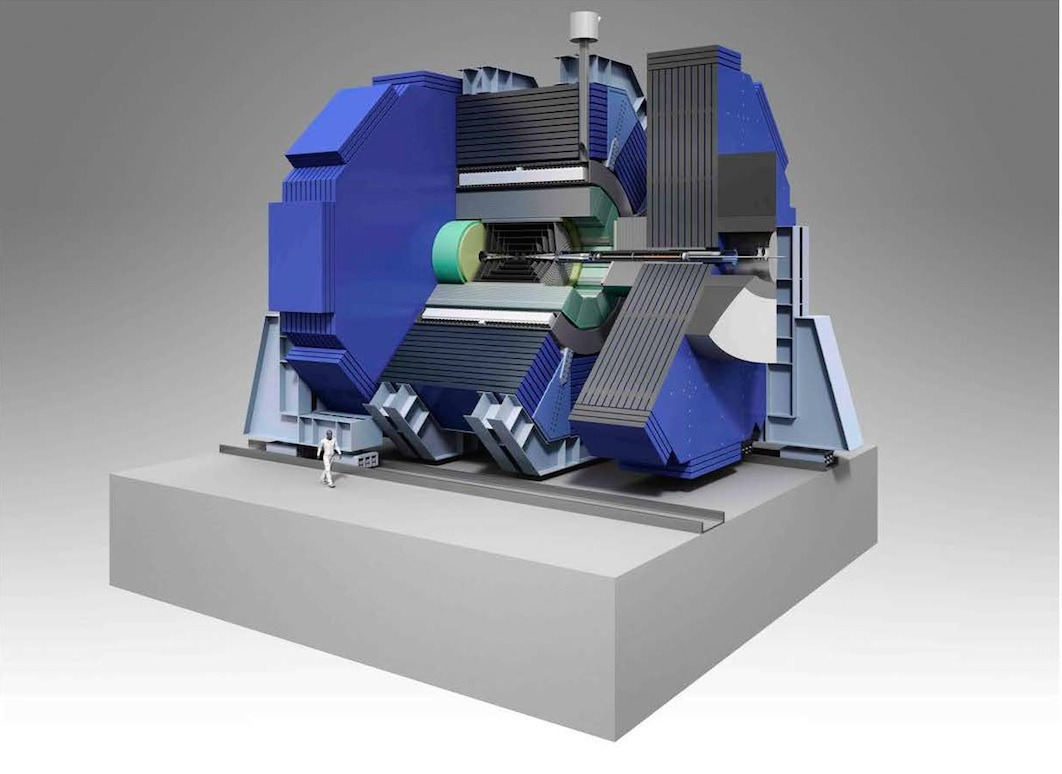
\includegraphics[width = \textwidth]{Pictures/ILC/SiD.jpg}
        \caption{\label{fig:SiD} The Silicon Detector}
      \end{subfigure}
      \begin{subfigure}[t]{0.5\textwidth}
        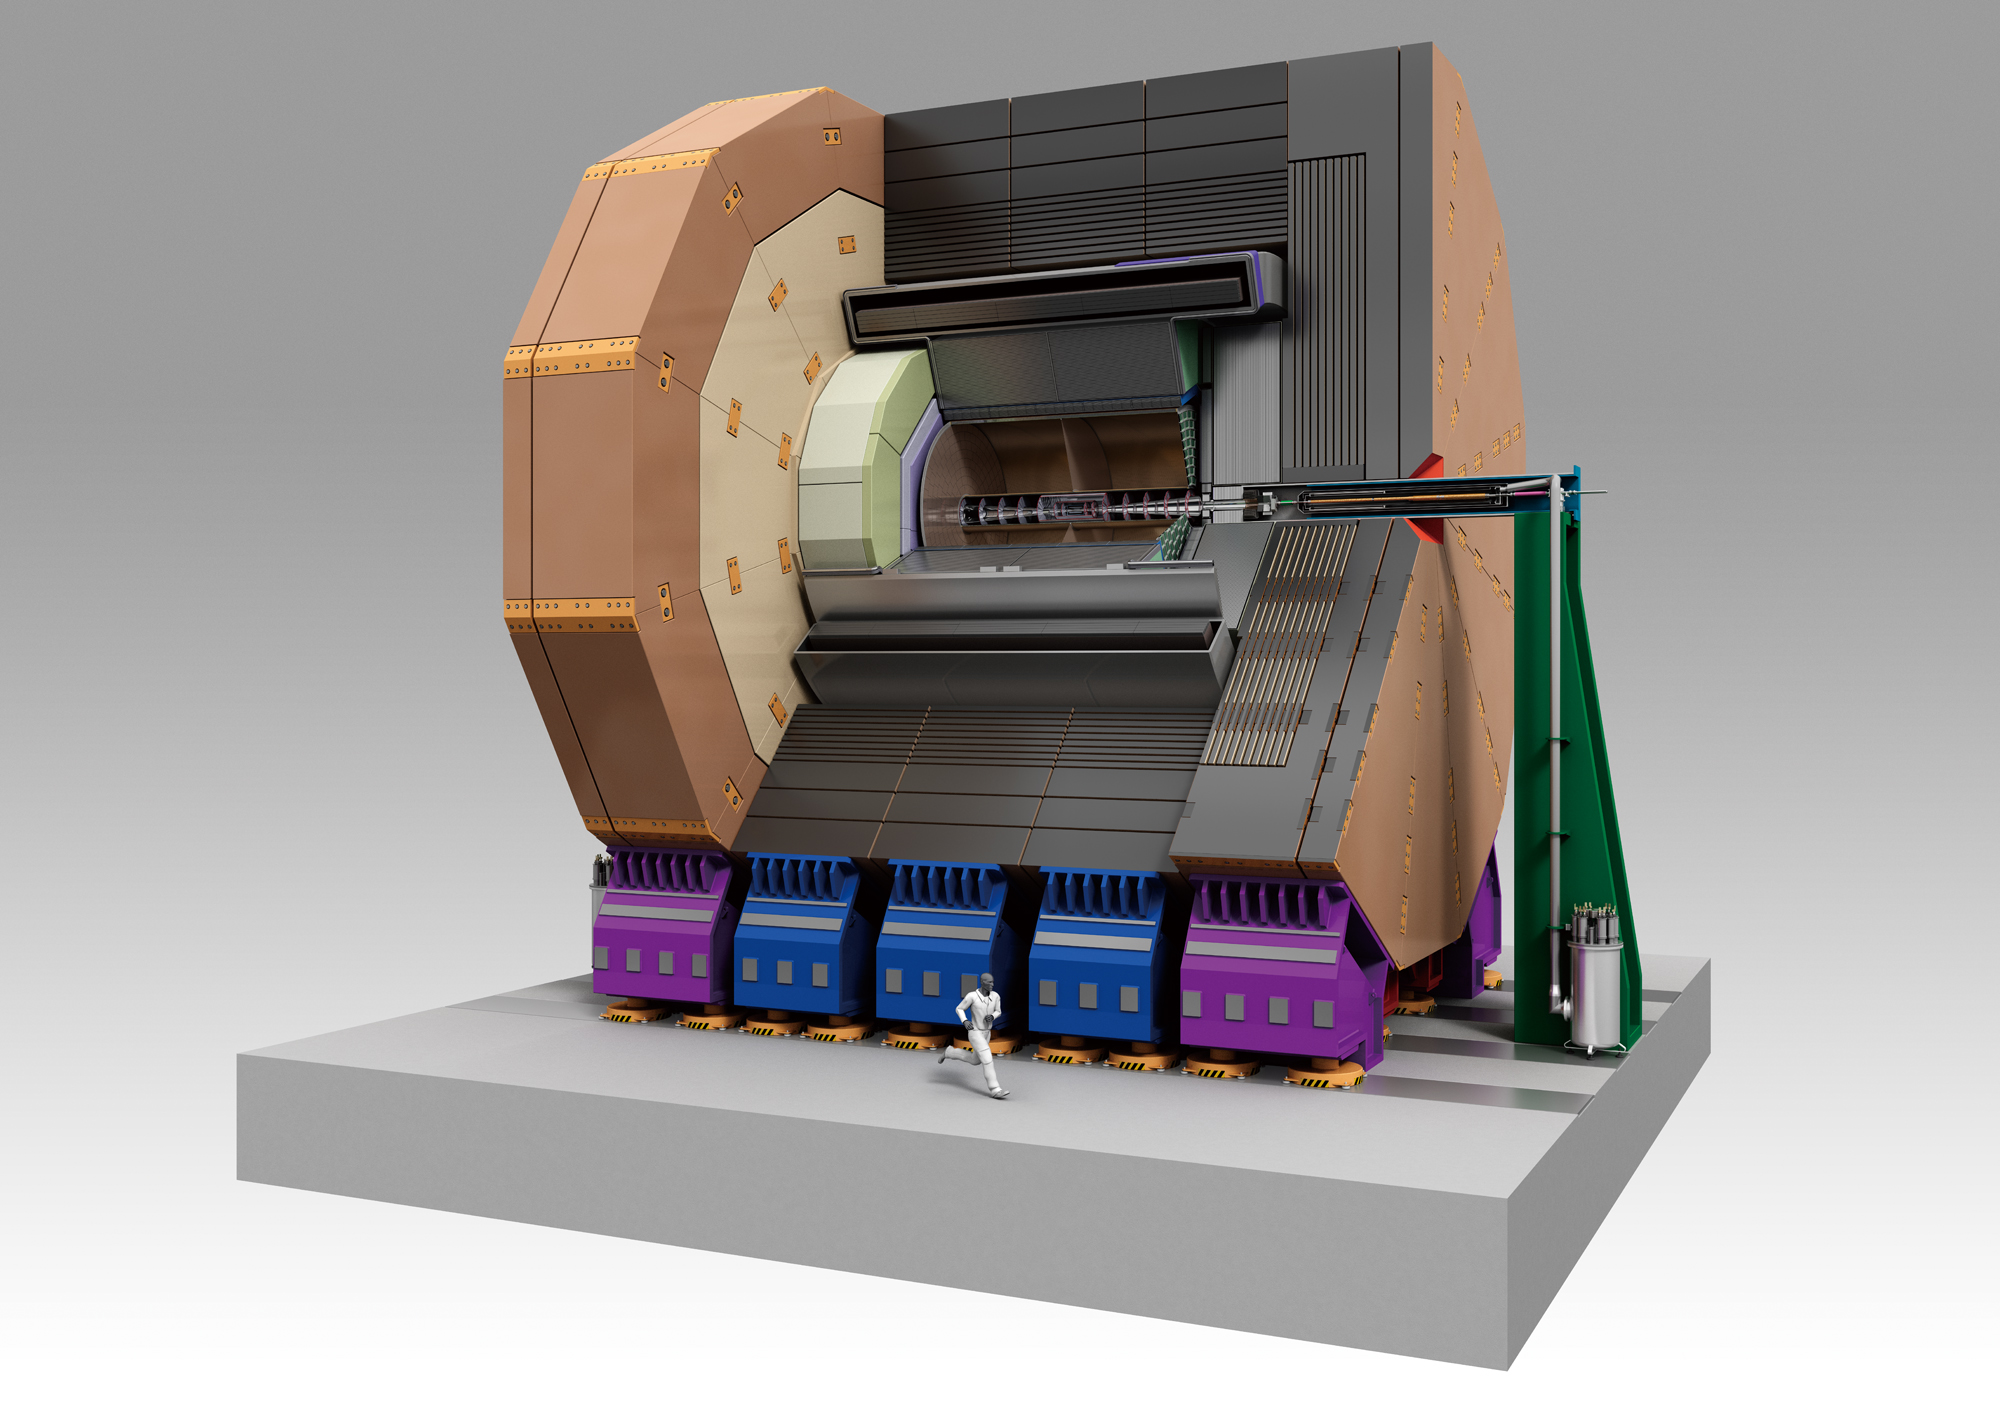
\includegraphics[width = 1.03\textwidth]{Pictures/ILC/ILD.jpg}
        \caption{\label{fig:ILD} The International Large Detector}
      \end{subfigure}
    \caption{Overview of the two detectors designs at the ILC. Fgure~(\subref{fig:SiD}) represents the SiD design while figure~(\subref{fig:ILD}) shows the ILD approach \cite{Behnke2010}.}
      \label{fig:Detectors}
    \end{figure}    

  As it was presented in section~\ref{subsec:design}, the \gls{ILC} will be built with only one interaction region due to cost reasons, whereas two detectors are foreseen.
  The push-pull operation scheme will allow for data taking of one detector, while the second one is out of the beam in a close-by cavern for maintenance.
  The interval to switch the detectors should be short enough and of the order of one day.
  This time efficient implementation sets specific requirements for the beam structure but also for the detector design.
  The detectors should be placed on platforms to preserve the alignment and to distribute the load equally onto the floor.
  Another requirement on the detector design is that the magnetic fields outside the iron return yokes must be small enough to not disturb the second detector on the parking position.
  It is assumed that a limit of $5~\rm{mT}$ at a lateral distance from the beam line should be sufficient.

  The motivation to build two detectors with a different approach is mainly to provide a cross-check and a confirmation of results and complementary strengths.
  Both detectors are optimised to study a broad range of precision measurements and search of new physics drove by the \gls{ILC} expectations.
  Their performances are driven by the \gls{PFA} to be able to measure the final states of events with a high accuracy.
  To do so, both detectors should have a high hermeticity, high granularity calorimeters and excellent tracking and vertexing.
  The \gls{PFA} is shortly presented on subsection~\ref{subsec:PFA}.

  The \gls{SiD} is a compact detector made of a silicon tracking and $5~\rm{T}$ magnetic field.
  The tracking system provides robust performance thanks to the time-stamping on single bunch crossings.
  The calorimeters are highly granular to perform the \gls{PFA}.

  The second detector is \gls{ILD}.
  In contrast to the \gls{SiD}, the tracking system is based on a continuous readout \gls{TPC} surrounded by silicon tracking detectors.
  The magnetic field will be only of 3.5 T combined with granular calorimeters for a good particle-flow reconstruction

    \subsection{Particle flow algorithm}
    \label{subsec:PFA}

    The main purpose of the \gls{ILC} (or the \gls{CLIC}) is to achieve precise measurements of physics processes that produce final states with multiple jets.
    The jet energy resolution at the \gls{ILC} should be sufficient to cleanly separate $W$ and $Z$ hadronic decays.
    Typically, the jet energy resolution is deduced from equation~\ref{eq:jet}, where $\alpha$ is the stochastic term usually greater than $\sim 60~\% / \sqrt{E\rm{(GeV)}}$.


    \begin{equation}
      \frac{\sigma_E}{E} \simeq \frac{\alpha}{\sqrt{E(GeV)}} \oplus \beta.
      \label{eq:jet}
    \end{equation}

    The \gls{PFA} approach is the extended version of the Energy Flow approach (used at H1, D0, CMS) for a highly granular detector. 
    The goal of this framework is to achieve a stochastic term for the energy resolution greater than $30~\% / \sqrt{E\rm{(GeV)}}$, not reachable with a traditional calorimeter.
    Each sub-detector should be efficient enough to separate and to reconstruct the four-vectors of all visible particles in an event.
    The energy of charged particle is measured in the tracking detectors, while the energy measurements for photons are done in the electromagnetic calorimeter and neutral hadrons are done in the hadron calorimeter.
    \todo{Why better? 60 \% tracks}
     
     \begin{figure}[!h]
      \centering
      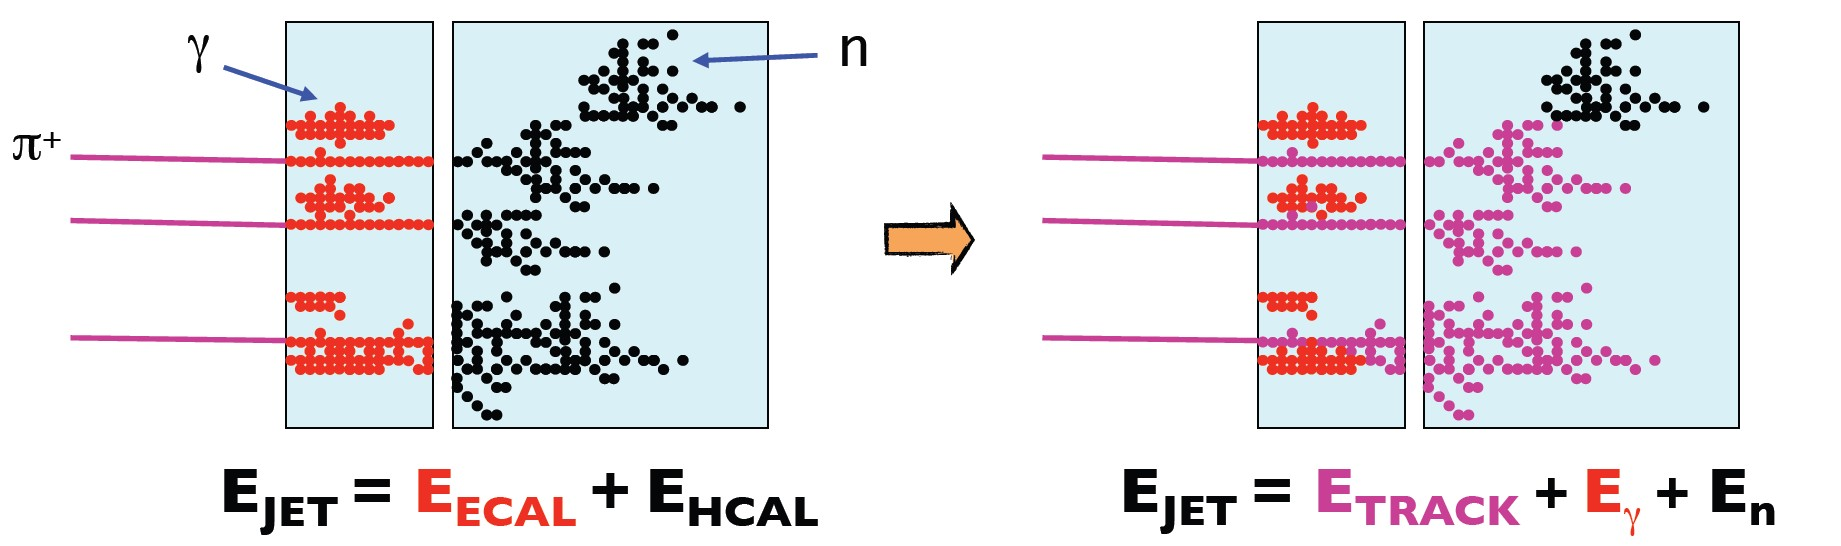
\includegraphics[width = 15cm]{Pictures/ILC/physics.jpg}
      \caption{Two different approaches for calorimetry. On the left is the traditional calorimetry method used on most of the experiments, the right one is the particle flow approach for calorimetry. The particle track is taken into account to calculate the jet energy \cite{PFA}.}
      \label{fig:jetEnergy}
    \end{figure}   
    
    The \gls{PFA} requirements drive the design of the detectors at the ILC.
    For both experiments, the electromagnetic and hadronic calorimeter have to be located inside the solenoid.
    Moreover, each sub-detector must be able to distinguish single particle signals, imposing a better tracking precision and higher granular calorimeters than the traditional detectors in high energy physics.

    \subsection{The ILD detector}
    \label{sec:ILD}
    
    \begin{figure}[!h]
      \centering
      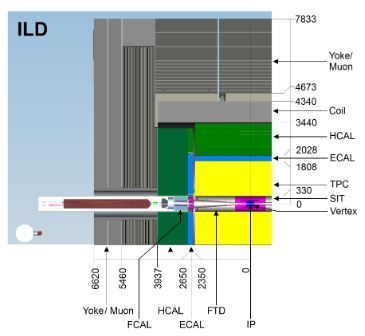
\includegraphics[width = 10cm]{Pictures/ILC/fig_ILD_Quadrant.png}
      \caption{Quadrant view of the ILD detector concept with its subdetector system \cite{Behnke2010}.}
      \label{fig:ILD_quadrant}
    \end{figure}

    The design of \gls{ILD} follows the requirements for optimal \gls{PFA} performance.
    In summary, the detector should be highly granular to have a robust three-dimensional imaging capability.
    It will combine a high-precision \acrfull{VXD} system, a hybrid tracking system and calorimeters inside a 3.5 T solenoid. 
    On the outside, a coil and iron return yoke will be instrumented as a muon system and a tail catcher.
    The figure~\ref{fig:ILD_quadrant} represents the different parts of the detector.

    The \gls{ILD} system coordinate is as following: the Cartesian coordinate system, where $x$ and $y$ are the horizontal and vertical coordiantes respectively, in the plane transverse to the beam line, while $z$ is along the beam line.
    For the spherical coordinate system, $r$ is the distance from the beam line, $\theta$ the track polar angle and $\phi$ the azimuthal angle.
    The third coordinate system is the cylindrical one.
    In this system, $r$ is the distance from the beam line, $\phi$ the azimuthal angle and $z$ the coordinate along the beam line.

      \subsubsection{Vertex detector}

      The \gls{VXD} is the closest detector to the interaction region and is in charge to measure particles' tracks and to reconstruct the decay vertices of the particles.
      For the moment, two vertex detector design are under study, but both of them have a pure barrel geometry.
      One geometry is made of five single sided layers, whereas the other one has three double-sided detection layers.
      Chapter~\ref{chap:vxd} will introduce in more details the vertex detector requirements for the \gls{ILD}, such as the material budget and the measurements precision aimed.
      The different design proposals will be presented. 

      \subsubsection{Tracking}

      The main tracking system for the \gls{ILD} is performed by the \gls{TPC}.
      It is a gaseous detector with a low material budget designed to measure the particles' trajectory.
      When a particle traverses through the \gls{TPC}, it ionises the gas, creating electrons that are drifting to the anode thanks to a high voltage.
      The anode is the part where the readout plates are installed.
      It provides a 3D position of the particles tracks thanks to the wires and the anode (give x-y) and the z coordinate is given by the drifting time.
      In addition to the exact position measurement, this detector is also able to measure the energy $\frac{dE}{dx}$ deposited by the particle, which can be used for particle identification.

      The requirements to design a \gls{TPC} at the \gls{ILC} are given by two main values: 
      
      \begin{itemize} 
        \item The single point resolution $\sigma_{s.p.}$ which should be lower than $100~\rm{\mu m}$ in the $r\phi$ direction and less than $500~\rm{\mu m}$ in the z direction;
        \item The minimum distance to separate two hits which should be lower than $2~\rm{mm}$.
      \end{itemize}

      The \gls{TPC} envisioned for \gls{ILD} is constituted of a central barrel part, with an inner radius of $\simeq 33~\rm{cm}$ and a outer radius of $\simeq 180~\rm{cm}$ and two endcaps with a detection area of $10~\rm{m^2}$. 
      The solid angle coverage is up to $|\cos{\theta} \simeq 0.98|$.
      The barrel will be filled with a gas mixture called T2K ($3~\%$ of Ar-CF4 and $2~\%$ of isobutane).
      Due to the low material budget and the ability to cope with a high magnetic field, the \gls{TPC} is compliant with the \gls{PFA} (see subsection~\ref{subsec:PFA}). 


      To improve the track reconstruction, the \gls{TPC} is surrounded by highly granular silicon detectors: two barrel components, the \gls{SIT} and the \gls{SET}; an end-cap component, the \gls{ETD} and the \gls{FTD}.
      The \gls{SIT} provides tracking between the \gls{VXD} and the \gls{TPC}, whereas the \gls{SET} is giving an entry point to the \gls{ECAL} after the \gls{TPC}.
      Both systems provide precise space points and improve the overall momentum resolution.
      The goal of the \gls{SIT} is to improve the momentum resolution, the reconstruction of low $p_{T}$ charged particles and the reconstruction of long-lived particles.
      The coupling of the \gls{SIT} and \gls{SET} provide also a time-stamping information.

      The \gls{ETD} is located within the gap separating the \gls{TPC} and the endcap calorimeter. 
      It improves the momentum resolution for charged tracks with a reduced path in the \gls{TPC}.
      It also reduces the effect of the material of the \gls{TPC} end-plate. 
      The material budget of this end-plate is estimated to $15~\%$ of $\rm{X_0}$.

      As the \gls{TPC} does not provide any coverage in the forward region, seven silicon disks ensure efficient and precise tracking down to very small angles, whereas the \gls{ETD} and the \gls{FTD} make sure to get a full tracking hermeticity.

      To simplify the system layout and the maintenance, the \gls{SIT}, \gls{SET} and \gls{ETD} are made of single-sided strip layers tilted by a small angle with respect to each other. 
      They are placed in a so-called false double-sided layers.
      The \gls{SIT} has two layers of microstrip, instead of one layer for the \gls{SET}. 
      The technology studied are microstrip sensors with an area of $10 \times 10~\rm{cm}^2$, with a pitch of $50~\rm{\mu m}$, a thickness of $200~\rm{\mu m}$ and an edgeless.
      The dead area of the sensors will be reduced down to few microns instead of $100~\rm{\mu m}$.
      The spatial point resolution aimed for this detectors is $\sim 7.0~\rm{\mu m}$ in the $r\phi$ direction.
      The table~\ref{tab:siTrackParam} gives the single point resolution aimed, as well as the angular coverage and the material budget.

      \begin{table}[!h]
        \centering
          \begin{tabular}{c K{2.5cm} c K{2.5cm}}
          \hline %----------------------------
          Detector &  Single point resolution ($\mu$m) &  Coverage  & Material budget $\rm{X_0}$ (\%) / layer\tabularnewline
          \hline %----------------------------
          \hline %----------------------------
          \multirow{2}*{SIT}  & $\sigma_{R-\phi} = 7.0 $  & \multirow{2}*{$\cos{\theta} \sim 0.91$ } & \multirow{2}*{0.65} \tabularnewline
                              & $\sigma_Z = 50.0 $ & & \tabularnewline
          SET      & $\sigma_R = 7.0$ & $\cos{\theta} \sim 0.79$ & 0.65 \tabularnewline
          ETD      & $\sigma_X = 7.0$ & $\cos{\theta} \sim 0.799 - 0.985 $ & 0.65 \tabularnewline
          \hline %----------------------------
          \end{tabular}
          \caption{Parameters aimed for the silicon tracker using micro-strips sensors.}
          \label{tab:siTrackParam}
      \end{table}

     The \gls{FTD} is placed in the forward direction, between the beam pipe and the inner field cage of the \gls{TPC}, where the magnetic field becomes less and less useful to bend charged tracks and so the determination of a precise momentum is more difficult.
     It consists of seven tracking disks: the two firsts are pixel detectors to cope with expected high occupancies and the five others are strip detectors.
     The pointing resolution will vary between $3.0-6.0~\rm{\mu m}$ for the two first layers and $7.0~\rm{\mu m}$ for the five other ones.
     

      \todo{Check the table and values....}

      \subsubsection{Calorimeters}

      The calorimeters design is driven by the particle flow requirements.
      Each particle must be reconstructed individually in the detector with a jet energy measurement equal to:
      \begin{equation}
        \frac{\Delta E}{E} = 30~\% / \sqrt{\frac{E}{GeV}}.
        \label{eq:jetRes}
      \end{equation}

      The energy resolution obtained in equation~\ref{eq:jetRes} is obtained thanks to a combination of information from the tracking system and the calorimeters. 
      The choice of technology used for the calorimeter will be determined by the pattern recognition performance. 
      One of the \gls{ILD} detector's goal is, for example, to be able to get a jet energy resolution sufficient to clean separate W and Z hadronic decays.
      
      The average jet energy distribution is roughly: 
      \begin{itemize}
        \item $62~\%$ are charged particles (mainly hadrons)
        \item $27~\%$ are $\gamma$
        \item $10~\%$ are long-lived neutral hadrons
        \item $1.5~\%$ are $\nu$
      \end{itemize}

      The \gls{ECAL} is the first calorimeter right after the tracking system.
      Its role is to identify photons and leptons and measure their energy, nevertheless, it is also the first section to develop the hadron showers.
      The fine segmentation makes an important contribution to hadron-hadron jet separation.
      For the \gls{ILD}, a compromise between the performance and the cost has led to use a sampling calorimeter realised with tungsten absorber.
      They are three options under study for the active area.
      The first one called SiW-ECAL, is made of silicon pin diodes with a pitch of $5 \times 5~\rm{mm}^2$. 
      It has the advantage to cover a large area, to be reliable and simple to operate, to have thin readout layers and can be operated in 3.5 T magnetic field.
      The second option is made of scintillator strips readout by photo-sensors and is called ScECAL.
      It has an active area of $5 \times 45~\rm{mm}^2$ arranged in alternative directions to achieve an effective granularity of $5 \times 5~\rm{mm}^2$ 
      The weakness of this technology happened in dense jets environment, where the reconstruction becomes more and more complicated.\todo{???}
      Some alternatives are also thought, like the Micromegas chambers. Nevertheless, this technology is less advanced compared to the others.
      One other good candidate could be the use of \gls{MAPS} sensors.
      They have the advantage to get the signal sensing and processing on the same  substrate and by choosing standard CMOS processes, the cost of fabrication would be reduced.

      The \gls{HCAL} has the role to separate the deposits energy of charged and neutral hadrons and to precisely measure the energy deposited.
      It is also a sampling calorimeter using stainless steel instead of tungsten as an absorber. 
      The rigidity of stainless steel makes possible to get a self-supporting structure limiting the dead areas.
      Two baseline technologies for the active medium area are studied.
      The  \gls{AHCAL} is made of scintillator tiles, whereas the semi-digital, called \gls{GRPC}, is based on the \gls{SDHCAL}.

      In order to monitor the luminosity and the beamstrahlung, the calorimeter system is completed in the very forward region by three different subsystems covering very small angles also for neutral hadrons: the LumiCal, the BeamCAL, and the \gls{LHCAL}.
      The LumiCAL is placed in a circular hole of the end-cap \gls{ECAL} and covers polar angles between 31 and 77 mrad. 
      It serves as luminosity monitor by measuring the Bhabha scattering $e^+e^- \rightarrow e^+e^-$ via emission of virtual $\gamma$.
      The luminosity $\mathcal{L}$ is determined by measuring  the ratio of the number of counted events $N_B$ in a considered polar angle ranged and the integral of the differential cross-section $\sigma_B$ in the same region.
      The measurement precision should be better than $10^{-3}$ at 500 GeV.
      After each bunch crossing, the beamstrahlung pairs hit the BeamCal.
      This would permit to get an estimation of the bunch-by-bunch luminosity, but also to determine the beam parameters.
      It is placed in front of the final focus quadrupole and covers polar angles between 5 and 40 mrad.
      The third system, the \gls{LHCAL}, ensure the coverage of the hadron calorimeter to small polar angles. \todo{WHY ?}

      \subsubsection{Magnetic Field and yoke}

     By applying a high magnetic field inside the detector, the charged particles have a bent track helping in the identification and the energy measurement.
     At the \gls{ILD}, the nominal magnetic field is 3.5 T and should have a high homogeneity inside the TPC.
     Moreover, as mentioned in subsection~\ref{subsec:design}, the magnetic beyond the coil has to be reduced to avoid any perturbations with the second detector in its parking position.
     A superconducting coil surrounding the tracking and calorimetric system generate the magnetic field.
     It has a diameter of 6.88 m, a length of 7.35 m and made of three modules.

     Surrounding the coil, an iron yoke ensures to return the magnetic flux. 
     It is constituted by a barrel of 2.88 m thickness and 2 end-caps of 2.12 m thickness.
     Muon detectors are inserted inside the iron yoke in a sandwich-like structure.
     They are performing measurement on muons but they are also used as tail catchers, to improve the energy resolution of high energetic jets escaping the calorimeters. 


   \section{Conclusions}

   The pros and cons of a linear collider using a electron/positron beam have been discussed. 
   The main advantage of this type of collider is to precisely know the initial collision state and to avoid any \gls{QCD} background contamination.
   Thus, precise measurements of the Higgs boson, such as a fine determination of its mass, its width and its couplings could be performed.
   Contrary to the \gls{LHC}, which is using the tunnel built for \gls{LEP}, the \gls{ILC} will be built on a new site.
   The tunnel, the accelerator, the detectors and the scientific campus have to be built. 
   To reduce the costs, only one interaction region is planned, on which two detectors are going to be operated alternatively.
   The design of these detectors is driven by the particle flow approach, which sets an energy resolution of $30~\%/\sqrt{E\rm{(GeV)}}$ for the calorimeters.
   The \gls{ILD} detector concept was introduced and the different sub-detectors and technology options were discussed, except for the vertex detector.
   The chapter~\ref{chap:vxd} is dedicated to the vertex detector at the \gls{ILD}.
   
   After describing the status of the \gls{SM} and the next high-energy experiment, the next chapter will introduce the physics cases at the \gls{ILC}, especially by describing an approach of a physics analysis to study the $H \rightarrow c\bar{c}$.

